\documentclass[a4paper,12pt]{article}

\usepackage[brazil]{babel}
\usepackage[utf8x]{inputenc}

\usepackage[a4paper,top=3cm,bottom=2cm,left=3cm,right=3cm,marginparwidth=1.75cm]{geometry}

\usepackage{amsmath}
\usepackage{graphicx}
\usepackage[colorinlistoftodos]{todonotes}
\usepackage[colorlinks=true, allcolors=blue]{hyperref}

\title{Relatório de Dados - Pelican Stores}
\author{Levy Marques Nunes}

\begin{document}
\maketitle

\section{Introdução}

Este relatório foi efetuado utilizando o conjunto de dados "PelicanStores.xlsx", disponibilizado no Ambiente Virtual de Aprendizado (AVA) pelo curso de Informática básica para estatística, com o professor e coordenador Bartolomeu Zamprogno. Utilizando o software $R$ para organizar, explorar e analisar estes dados, pude concluir os fatos abaixo apresentados.
\\
\\
\\
\\

\section{Sobre o Conjunto de Dados Pelican Stores}

\subsection{Variáveis}

O conjunto de dados possui 8 variáveis:
\begin{enumerate}
\item Cliente (inteiro)
\item Tipo de cliente (fator)
\item Quantidade de itens comprado por cada cliente (inteiro)
\item Vendas Líquidas (numérico)
\item Método de Pagamento (fator)
\item Gênero do cliente (fator)
\item Estado civil do cliente (fator)
\item Idade do cliente (inteiro)
\end{enumerate}

\subsection{Resumo do conjunto de dados}
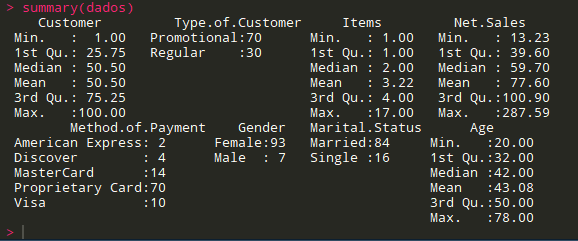
\includegraphics{resumo.png} \\

Como podemos observar pela imagem acima, as variáveis descritas como fatores, tiveram suas informações mostradas como uma tabela de valores, enquanto as variáveis inteiras e numéricas foram apresentadas com estatísticas próprias (Como quantis, médias, máximos e mínimos).\\

\section{Relatório Gerencial - Questão 1}
Distribuição de frequências relativas das principais variáveis.

\subsection{Tipo de cliente}
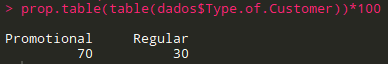
\includegraphics[]{tipo.png}\\

Usando o comando ''prop.table'' do $R$, podemos obter uma tabela das frequências relativas em formato decimal, para obter a porcentagem, multiplica-se por 100. Com isso, podemos ver claramente que o conjunto de dados Pelican Stores possui quase $3/4$ de sua clientela formada por clientes promocionais.\\

\subsection{Item}
Variável referente ao número de itens comprados por cada cliente.\\
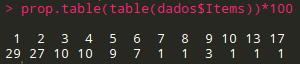
\includegraphics[]{item.png}\\
Podemos ver nesta tabela de proporções que a maioria dos clientes costuma comprar poucos itens, veja que é raro ver clientes comprando mais do que 6 itens.\\

\subsection{Vendas líquidas}
A quantia total (em dólares) cobrada pelo cartão de crédito.\\
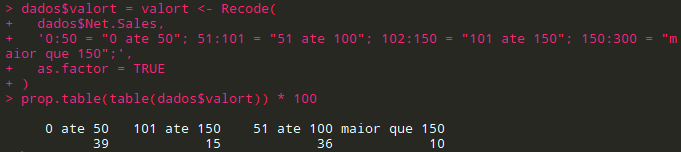
\includegraphics[]{valor.png}

Como a variável ''Vendas líquidas'' é numérica, ou seja, quantitativa contínua, tive que organizar em pequenos intervalos, igual a um histograma.
Usando a função ''Recode'' do pacote ''car'' do $R$, pude redefinir os valores em uma nova variável ''valort'' (valor tabelado). Essa nova variável guarda os valores contínuos em forma de fatores.\\
Veja que a maioria das compras (mais de 70\%) são efetuadas com valores menores do que 100 dólares.\\

\subsection{Método de pagamento}
Qual forma de pagamento o cliente utilizou para efetuar a compra.\\
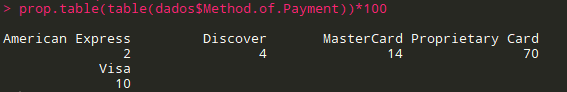
\includegraphics[]{metodo.png}\\

Veja que o ''Proprietary Card'' é de longe o mais utilizado pelos clientes, seguido pelo cartão ''MasterCard'', e pelo cartão ''Visa''.\\

\subsection{Gênero}
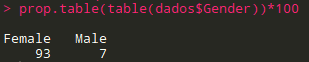
\includegraphics[]{genero.png}\\

Podemos ver que uma maioria esmagadora dos clientes são mulheres (mais de 90\%).

\subsection{Estado civil}
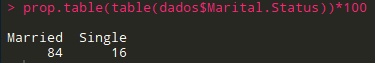
\includegraphics[]{casamento.png}\\
Acima, podemos observar que mais de 80\% dos clientes são casados.

\subsection{Idade}
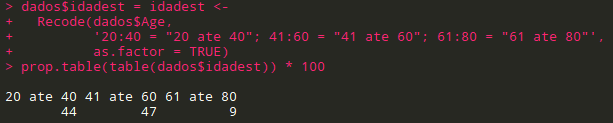
\includegraphics[]{idade.png}\\

O mesmo caso da variável ''Vendas líquidas'', mas desta vez é uma quantitativa discreta.\\

Podemos observar que os clientes estão dispersadamente distribuidos entre 20 e 60 anos.

\section{Questão 2}
Um grafico de colunas ou gráfico de setores mostrando o número de compras de clientes atribuíveis ao método de pagamento.\\
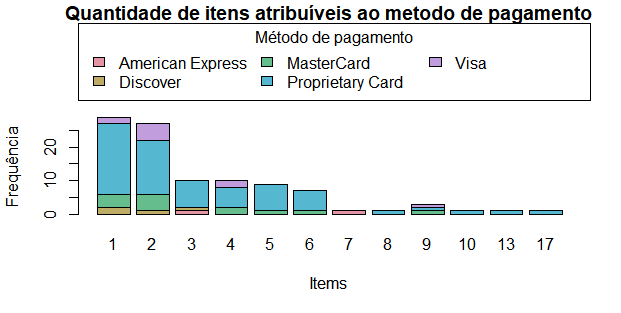
\includegraphics[]{ave.png}\\

Como já vimos na variável método de pagamento, o cartão ''Proprietary Card'' é usado por 70\% dos clientes, então é normal que seja usado independente do número de itens. Mas o que é interessante de fato, é a utlização do cartão ''Visa'' e do ''MasterCard'', que têm seu uso reduzido a maneira que a quantidade de itens aumenta.\\
\\
\\
\\
\\

\section{Questão 3}
Uma tabulação cruzada do tipo de cliente (regular ou promocional) \textit{versus} as vendas líquidas.\\
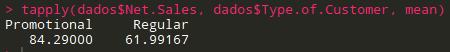
\includegraphics[]{tapply.png}\\

Como existem bem mais clientes promocionais do que regulares, não faria sentido comparar a soma dos valores de cada tipo de cliente, obviamente os promocionais compraram mais. Então utilizei uma medida de tendência central como forma de normalizar essa diferença.\\
Perceba que os clientes promocionais gastam, em média, 20 dólares a mais do que os clientes regulares.\\

\section{Questão 4}
Um diagrama de dispersão para explorar a relação entre vendas líquidas e idade do cliente.\\
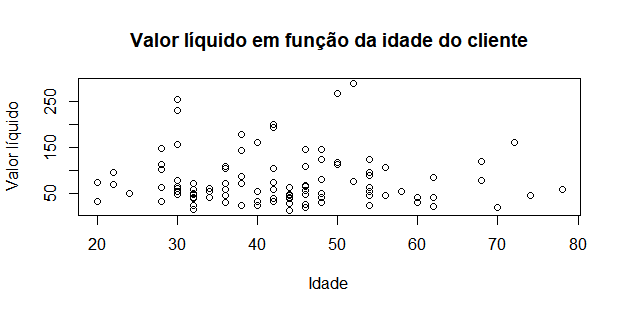
\includegraphics[]{valorl.png}\\

Como podemos observar acima, a nuvem de pontos está muito dispersa, e não conseguimos perceber uma relação linear positiva e nem negativa neste gráfico.\\

Então é seguro dizer que a variável ''Valor líquido'' e ''Idade'', não se correlacionam neste conjunto de dados.

\end{document}